\subsection{Falling blocks}\label{sec:block}
This benchmark is described as proposed by \citet{Gerya2003a}, \citet{Gerya2010} and \citet{Thieulot2011}. The domain is square with $L_x=L_y=$ \SI{500}{\km}
and the grid is composed by $50\times50$ elements with 25 markers in each element. The block is initially centred at ($x=$ \SI{250}{\km}; $y=$ \SI{400}{\km})
and has a size of $100\times100$ km (Fig. \ref{fig:block}a). The fluid surrounding the block has $\eta_f=$ \SI{e21}{\pascal\per\s} and $\rho_f=$
\SI{3200}{\kg\per\cubic\m}. The benchmark tests with different viscosities of the block, with $\eta_b$ from \SIrange{e15}{e27}{\pascal\per\s}. In each
experiment also the density $\rho_b$ of the block varies from \SIrange{3220}{9900}{\kg\per\cubic\m}. Velocity boundary conditions are set to free slip
conditions on all sides of the domain. Density distributions at $t=$ \SI{20}{\mega\year} for $\rho_b=$ \SI{3300}{\kg\per\cubic\m} and different $\eta_b$
are plotted in Fig. \ref{fig:block}b-f, showing that the code correctly preserve the block geometry in case of large viscosity contrast, with a block stiffer
than the surrounding fluid (Fig. \ref{fig:block}f).

The velocity in the centre of the falling block at $t=0$ is measured for all experiments and, since the velocity should increase with density contrast, the
quantity $\bm{v}/(\rho_b-\rho_f)$ is plotted as function of the viscosity contrast. All results perfectly match with those from \citet{Gerya2010} and they
line up on a single curve, demonstrating that the code can correctly deal with large viscosity and density contrasts (Fig. \ref{fig:falling}). All data can be 
found at \url{https://github.com/aleregorda/Benchmarks/tree/main/Momentum_equation/Falling%20blocks}.

\begin{figure}
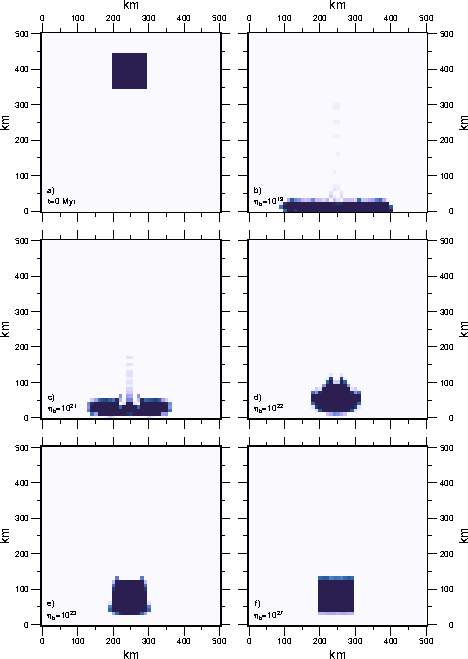
\includegraphics[width=300px]{./Figures/Block.pdf}
\centering
\caption{Density evolution of the falling block experiment at $t=$ \SI{0}{\mega\year} (panel a) and $t=$ \SI{20}{\mega\year} for different viscosities of the
block (panels b-f).}
\label{fig:block}
\end{figure}

\begin{figure}
\centering
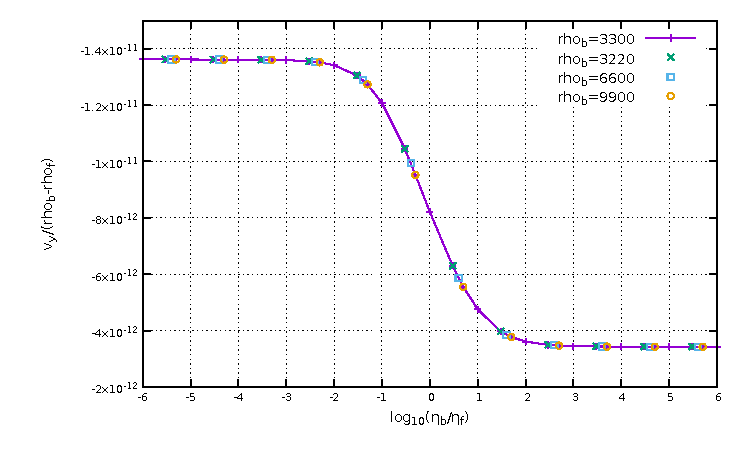
\includegraphics[width=400px]{./Figures/Falling.pdf}
\caption{Initial velocity relative to the density contrast at the centre of the falling block as function of the viscosity contrast between the block and the
surrounding fluid.}
\label{fig:falling}
\end{figure}